%!TEX program = xelatex
%%%%%%%%%%%%%%%%%%%%%%%这是导言部分的开始%%%%%%%%

%========= 导言部分声明文档的类型=================
\documentclass{article}

	%=========导言部分可可以加载宏包=================
	\usepackage{amsmath}                % 数学公式排版宏包
	\usepackage{amssymb}                % 数学符号命令宏包
	\usepackage{amsthm}                 % 数学定理宏包
	\usepackage[UTF8]{ctex}             % 中文输入宏包
	\usepackage[a4paper]{geometry}      % 页面设置宏包
	\usepackage{setspace}               % 行间距宏包
	\usepackage{graphicx}               % 图片宏包
	\usepackage{listings}               % 代码宏包
	\usepackage{color}					% 颜色宏包
	\usepackage{xcolor}                 % 颜色处理宏包
	\usepackage{float}                  % 浮动对象式样宏包
	\usepackage{fontspec}
	\usepackage{enumerate}				% 列举编号包
	
	%=========页面设置==============================
	\geometry{left=1cm,right=1cm,top=1cm,bottom=2cm}
	\onehalfspacing
	\setlength\parindent{0em}

	%=========代码格式设置============================
	\definecolor{dkgreen}{rgb}{0,0.6,0}
	\definecolor{gray}{rgb}{0.5,0.5,0.5}
	\definecolor{mauve}{rgb}{0.58,0,0.82}
	% \setmonofont{Consolas}
	\lstset{
		numbers = left, 	
		numberstyle = \color{gray}, 
		keywordstyle = \color{blue},
		commentstyle = \color{dkgreen}, 
		stringstyle = \color{mauve},
		basicstyle = \ttfamily,
		breaklines = true,
		frame = shadowbox, % 阴影效果
		rulesepcolor = \color{ red!20!green!20!blue!20} ,
		escapeinside = ``, % 英文分号中可写入中文
		xleftmargin = 2em,xrightmargin=2em, aboveskip=1em,
		framexleftmargin = 2em
	} 

%=========导言部分可以定义标题信息===============
\title{组会报告}
\author{徐益}
\date{\today}
%%%%%%%%%%%%%%%%%%%%%%%这是导言部分的结束%%%%%%%%%

%%%%%%%%%%%%%%%%%%%%%%%这是正文部分的开始%%%%%%%%%
\begin{document}

%=========生成标题================================
\maketitle

%=========开始正文的输入==========================

%===========第一节=================
\section{工作内容}
1. 完成LDPC-mex-sim

2. 阅读Intel® 64 and IA-32 Architectures Software Developer’s Manual Volume 1

3. 学习Intrinsics Guide并测试

%===========第一节=================
\section{SIMD(single instruction, multiple data)}
\subsection{SIMD Execution Model}
\begin{figure}[H]
	\centering
	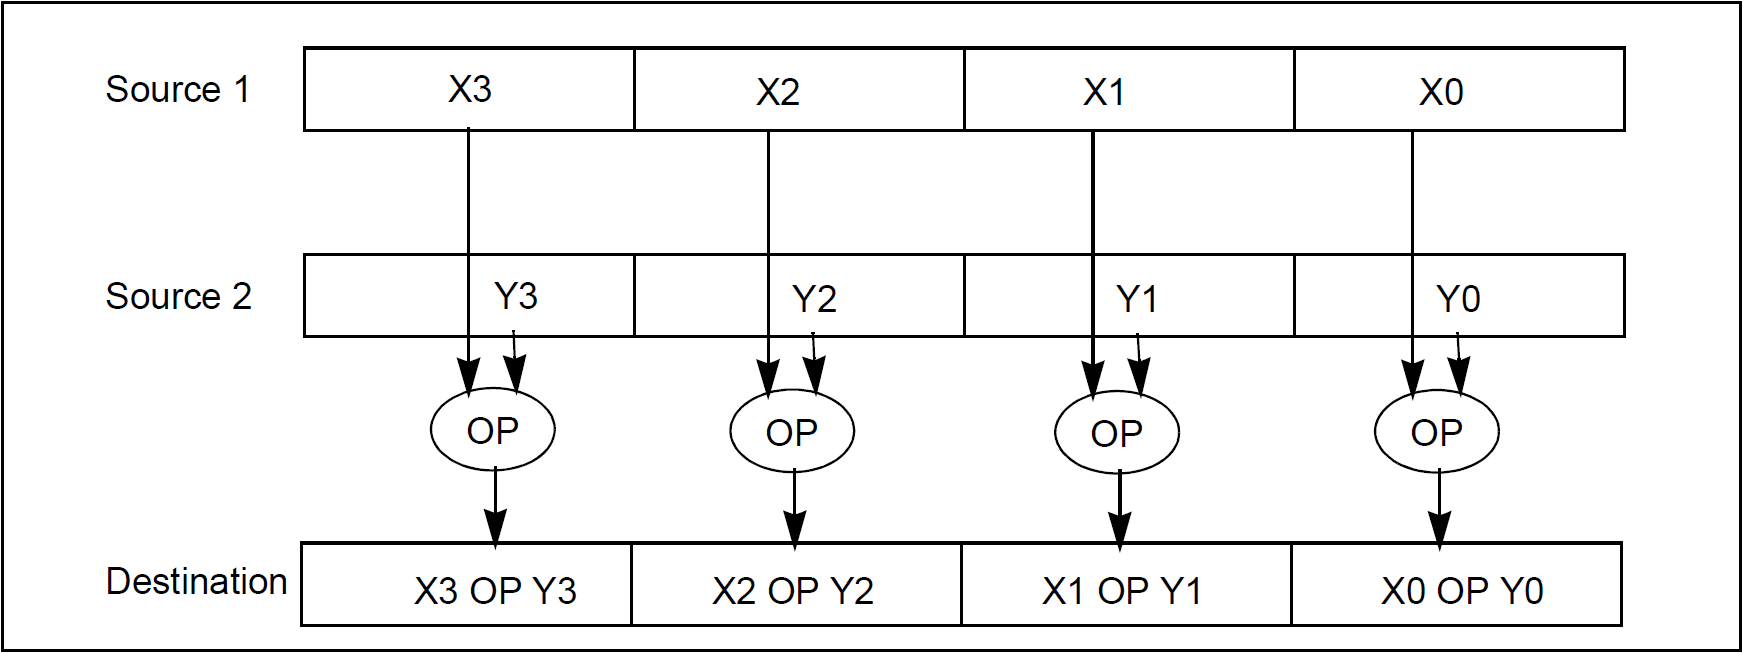
\includegraphics[width = .8\textwidth]{SIMD_Execution_Model.png}
	\caption{SIMD Execution Model}
\end{figure}
\begin{figure}[H]
	\centering
	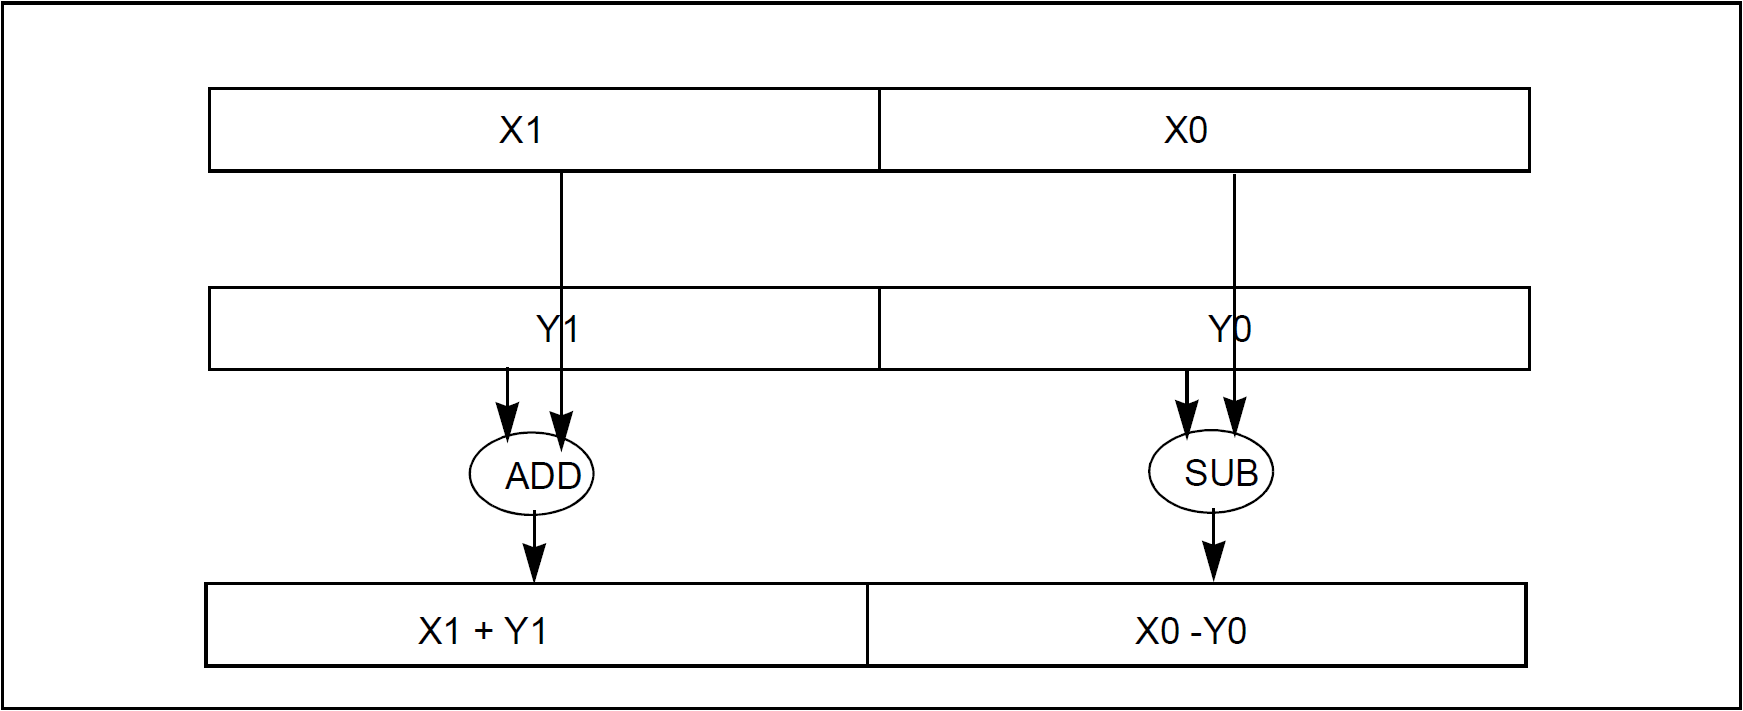
\includegraphics[width = .8\textwidth]{Asymmetric_Processing_in_ADDSUBPD.png}
	\caption{Asymmetric Processing in ADDSUBPD}
\end{figure}
\begin{figure}[H]
	\centering
	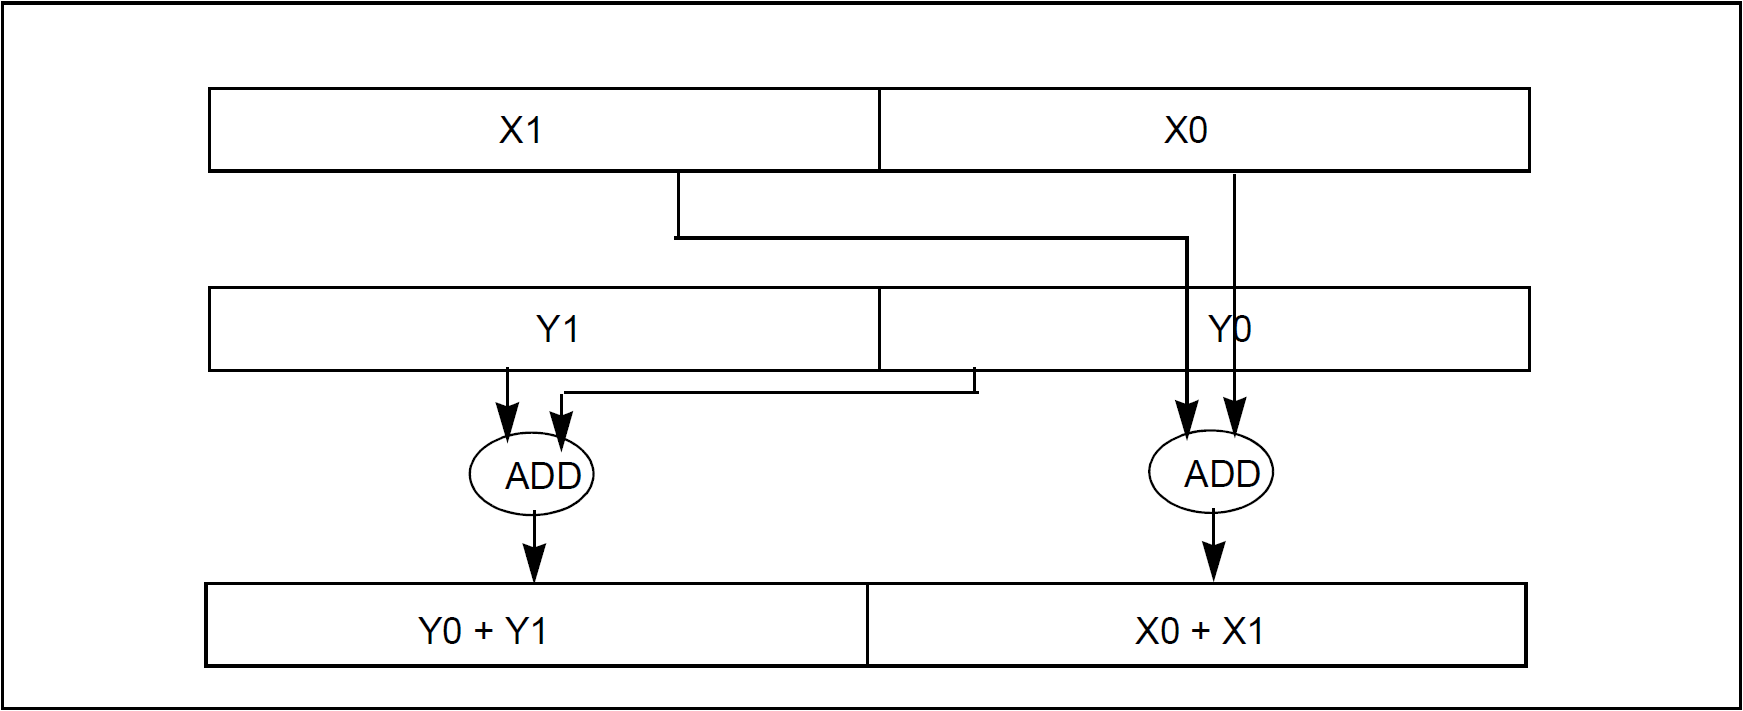
\includegraphics[width = .8\textwidth]{Horizontal_Data_Movement_in_HADDPD.png}
	\caption{Horizontal Data Movement in HADDPD}
\end{figure}
\subsection{SIMD Execution Environment}
\begin{figure}[H]
	\centering
	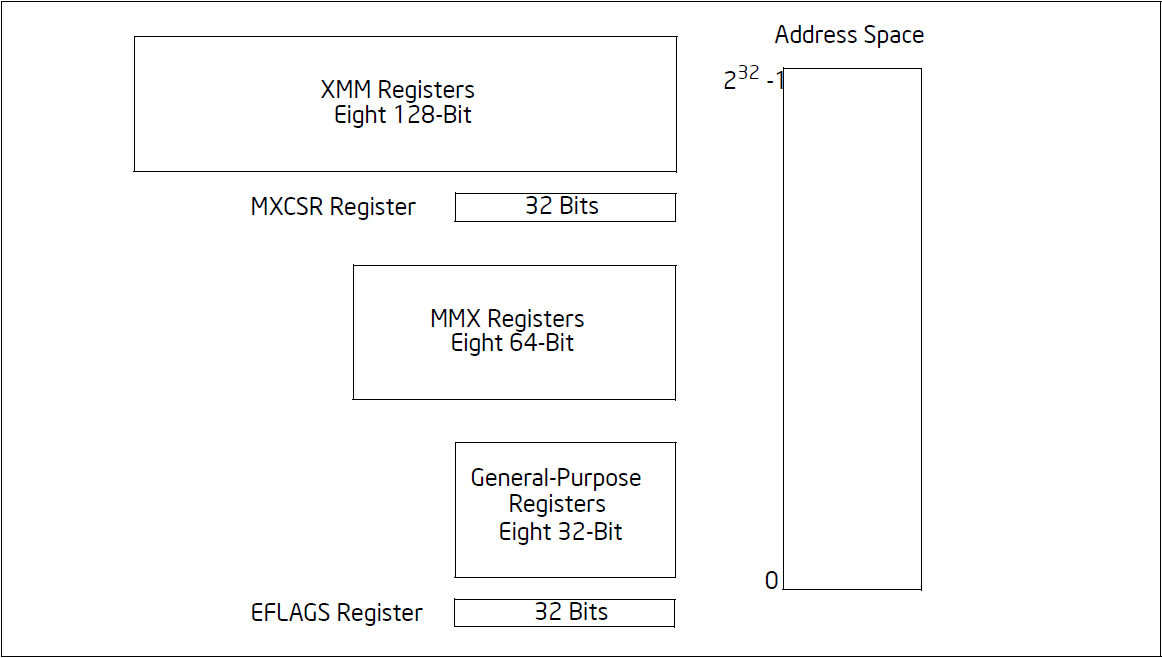
\includegraphics[width = .7\textwidth]{SSE_Execution_Environment.png}
	\caption{SSE Execution Environment}
\end{figure}
\begin{figure}[H]
	\centering
	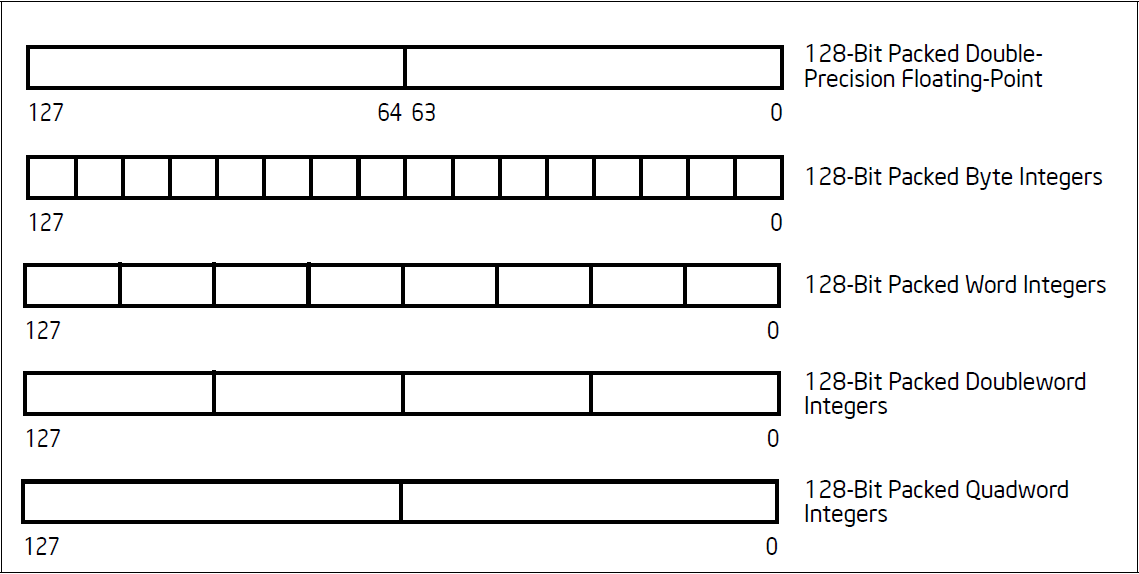
\includegraphics[width = .7\textwidth]{Data_Types_Introduced_with_the_SSE2_Extensions.png}
	\caption{Data Types Introduced with the SSE2 Extensions}
\end{figure}
\begin{figure}[H]
	\centering
	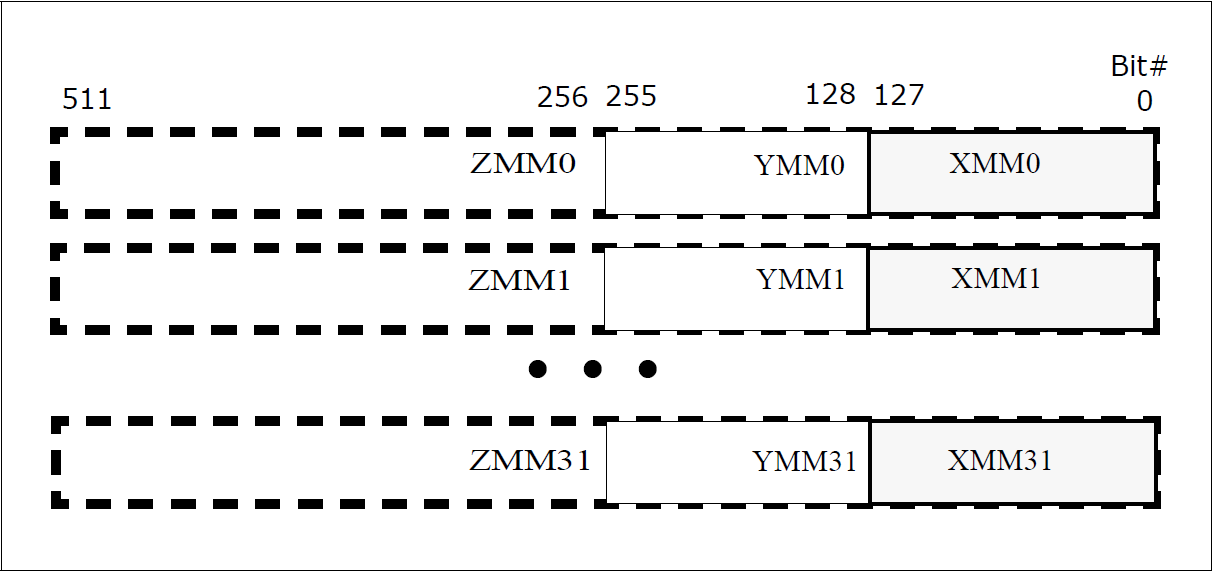
\includegraphics[width = .8\textwidth]{ZMM.png}
	\caption{AVX-512 ZMM}
\end{figure}
\begin{figure}[H]
	\centering
	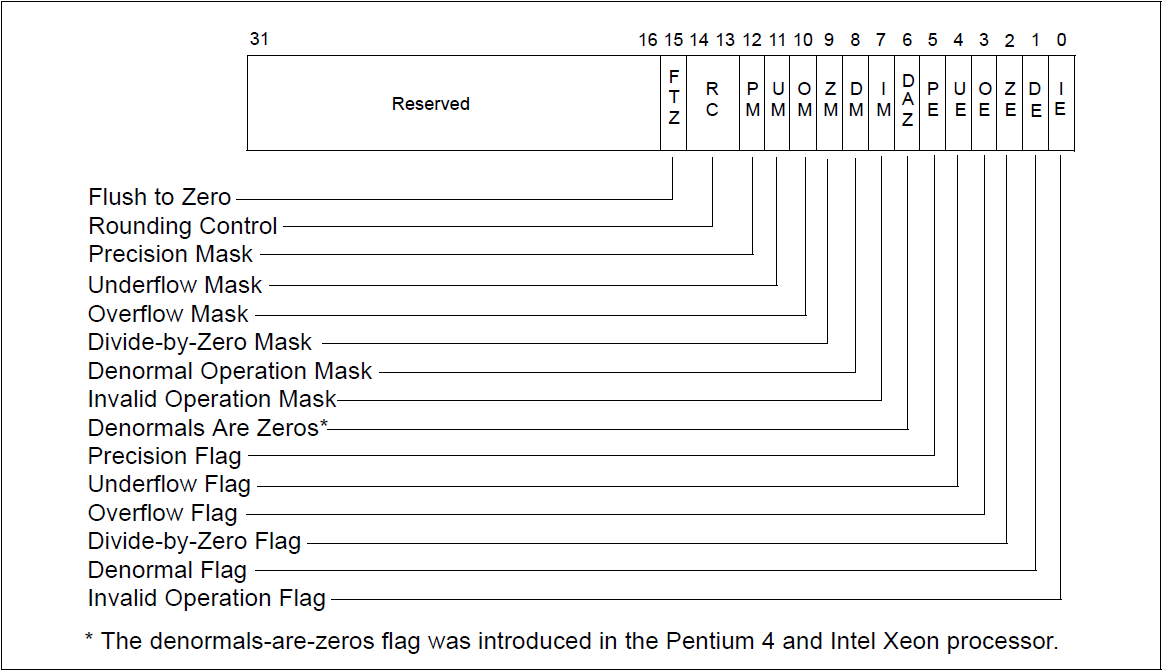
\includegraphics[width = .8\textwidth]{MXCSR.png}
	\caption{MXCSR}
\end{figure}
\begin{figure}[H]
	\centering
	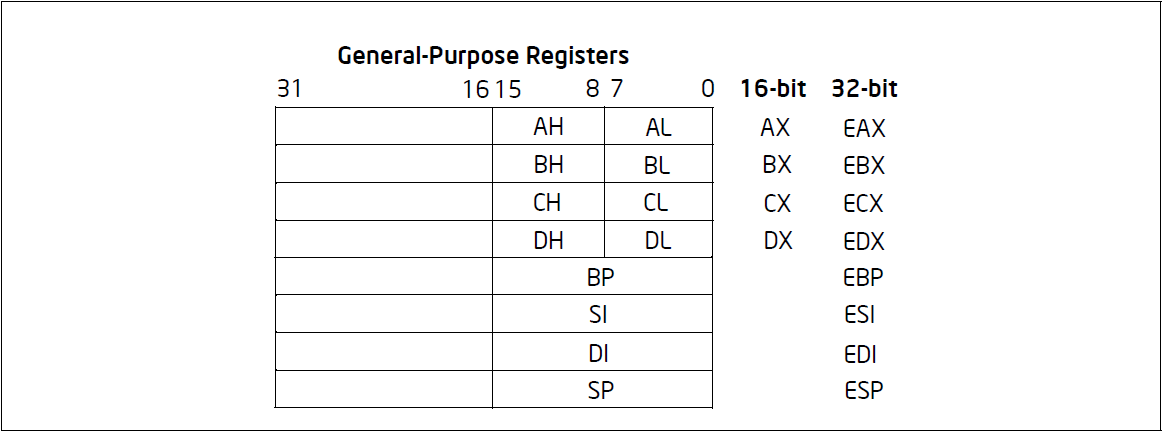
\includegraphics[width = .8\textwidth]{General-Purpose_Register.png}
	\caption{General-Purpose Register}
\end{figure}
\begin{figure}[H]
	\centering
	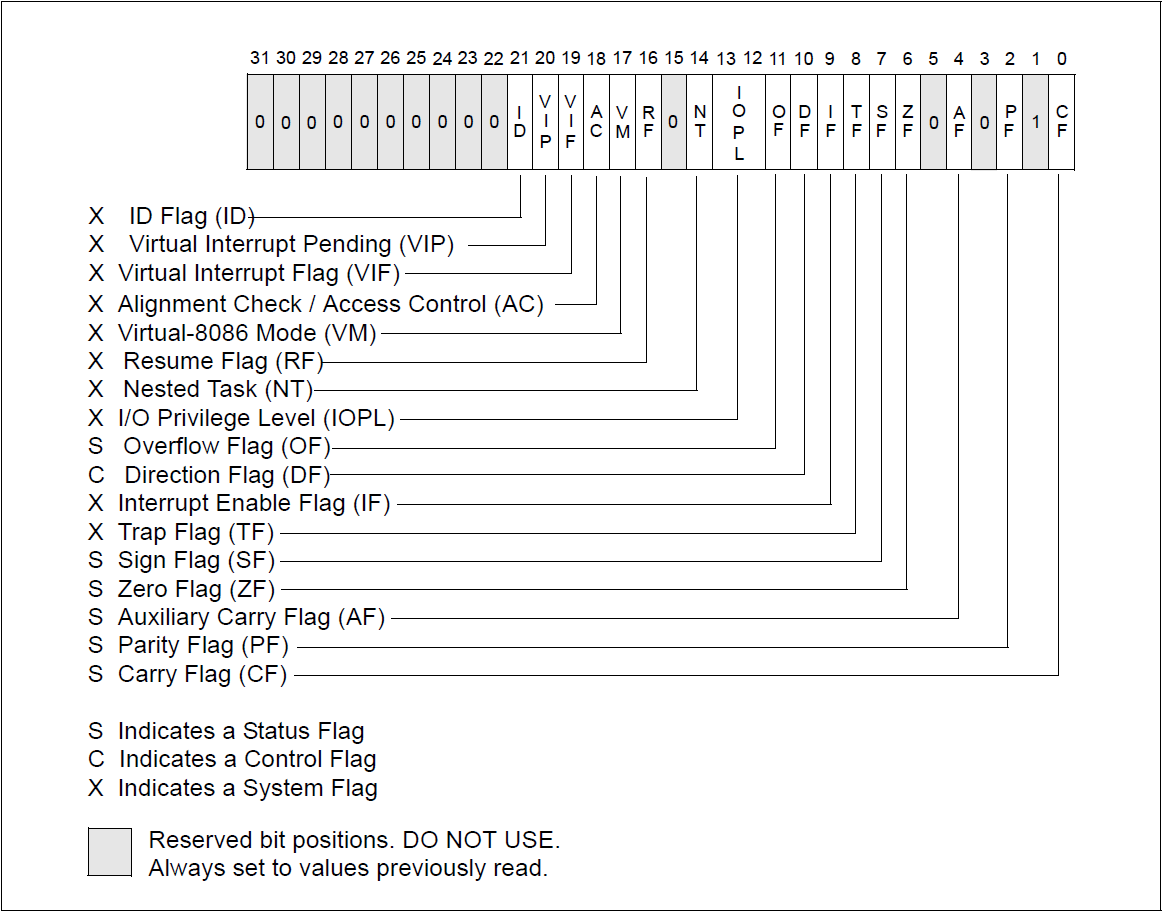
\includegraphics[width = .8\textwidth]{EFLAG.png}
	\caption{EFLAG}
\end{figure}

%===========第二节=================
\section{Intrinsics Guide测试}
\subsection{测试函数}
\lstset{language=C++}
\begin{lstlisting}
#include <immintrin.h>
/* 32个int8_t并行相加 */
void simd_add_int8_32(int8_t* a, int8_t* b, int8_t* r)
{
	__m256i mma, mmb, mmr;
	/* load */
	mma = _mm256_load_si256((__m256i*)a);	// vmovdqa ymm, m256
	mmb = _mm256_load_si256((__m256i*)b);
	/* add */
	mmr = _mm256_add_epi8(mma, mmb);	// vpaddb ymm, ymm, ymm
	/* store */
	_mm256_store_si256((__m256i*)r, mmr);	// vmovdqa m256, ymm
}
/* 8个float并行相加 */
void simd_add_float_8(float* a, float* b, float* r)
{
	__m256 mma, mmb, mmr;
	/* load */
	mma = _mm256_load_ps(a);		// vmovaps ymm, m256
	mmb = _mm256_load_ps(b);
	/* add */
	mmr = _mm256_add_ps(mma, mmb);		// vaddps ymm, ymm, ymm
	/* store */
	_mm256_store_ps(r, mmr);		// vmovaps m256, ymm
}
\end{lstlisting}
\subsection{耗时测试}
\begin{table}[H]
	\caption{3.2E7次加法运算耗时(VS compiler)}
	\centering
	\begin{tabular}{|l|l|l|l|}% 通过添加 | 来表示是否需要绘制竖线
		\hline  % 在表格最上方绘制横线
		数据类型 & SIMD		& 非SIMD  \\
		\hline
		int8\_t	& 3.367s	& 8.496s \\
		\hline
		float	& 12.341s	& 7.676s \\
		\hline  % 在表格最下方绘制横线
	\end{tabular}
\end{table}
\begin{table}[H]
	\caption{3.2E7次加法运算耗时(Intel C++ compiler)}
	\centering
	\begin{tabular}{|l|l|l|l|}% 通过添加 | 来表示是否需要绘制竖线
		\hline  % 在表格最上方绘制横线
		数据类型 & SIMD		& 非SIMD  \\
		\hline
		int8\_t	& 3.045s	& 8.081s \\
		\hline
		float	& 12.272s	& 7.409s \\
		\hline  % 在表格最下方绘制横线
	\end{tabular}
\end{table}

%===========第三节=================
% \section{测试LDPC速率匹配模块}

%===========第四节=================
% \section{仍存在问题}

%===========下周计划=================
% \section{下阶段计划}
% 实现LDPC剩余的mex函数

\end{document}
%%%%%%%%%%%%%%%%%%%%%%%这是正文部分的结束%%%%%%%%%%%%